
\chapter{Simulation}
\label{chap:simulation}
%TODO: Reformulate
As mentioned previously in this paper, there are many advantages to performing simulation vs. carryings 


The simulation environment, hereafter referred to as simple \textit{the simulation}, will be the abstract platform on which the quadcopters and their control algorithm can be tested. 
In this chapter i will outline the construction of the simulation platform, as well of the validation used to ensure that the simulation follows the required physical mechanics. 

\section{Simulation vs. Animation}
\label{sec:simulation_animation}

%TODO mention importance of distribution

\section{Software}
The software used in this paper to create the simulation platform is Matlab Version 8.7 (R2016a) with Simulink \cite{_matlab_2016}. Simulink was chosen based on its ease of use and ability to perform simulations continuous time. Simulink also has a 3D graphics engine called \texttt{VR3D}\cite{_matlab_2016}, which can be used to model 3D animations from any signal output from the simulation model. I.e. if the simulation models a flying quadcopter, the position values of the quadcopter can be sent as signals to the 3D model. The ability to 3D animate the movements of the quadcopters is important, as \textit{seeing} their actual flight paths can be a simple way to discover errors in either the simulation model or the control algorithm. 

\section{Design}
\label{sec:design}
This section will outline the specifications of the simulation platform, after which it is designed. Please note that some specifications were not intended from the beginning, such as a limitation on global velocity, but are the result of an iterative design process and tuning the simulation. 

\subsection{Control Problem}
\label{sec:control_problem}
The goal of the control problem is to challenge the control algorithms such that they can be compared. The control problem chosen for the purpose of this thesis, will be for the agents to collaborate on assembling a structure. The structure will be made of boxes or bricks (hereafter referred to only as boxes), which the agents are able to lift and relocate. The starting position of the boxes will be in one end of the rectangular environment, where the assembled structure will be in the other end. This type of setup requires movement by the agents in close proximity to each other, which introduces the risk of collision. This type of problem must also be solved in a specific order, such that the bottom of the structure is created first etc.
The control algorithm will be given the position of boxes as well as the position for the proposed bricks in the completed structure.
The measurements used to test the performance of the control algorithm on this problem are outlined in \ref{sec:test_metrics}. Figure \ref{fig:2d_overview} shows the design of the simulation environment, with the control problem and the agents viewed from the top.

% Control problem
\begin{figure}[H]
  \centering
  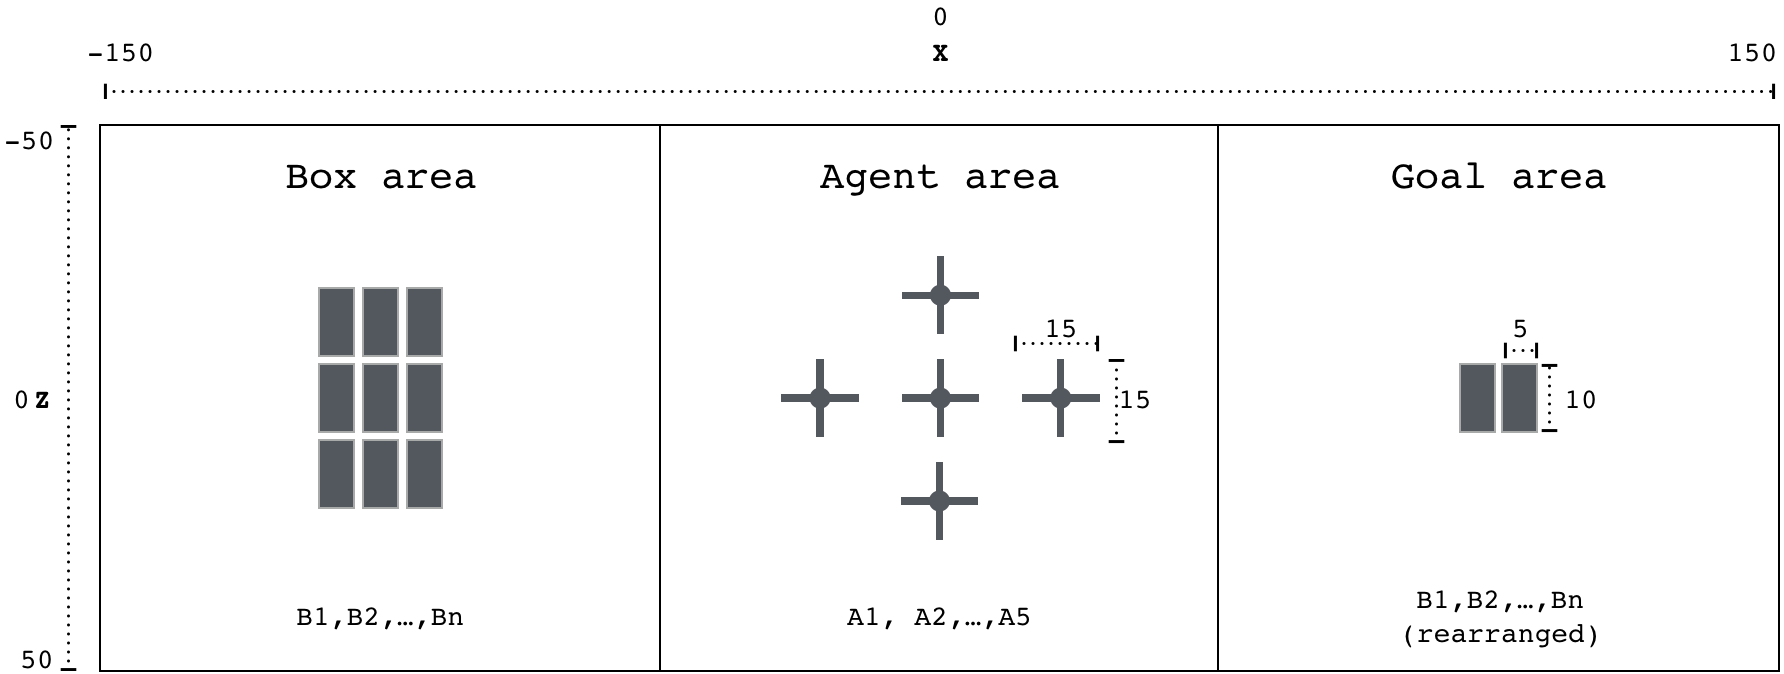
\includegraphics[width=1\columnwidth]{figures/2d_overview}
  \caption{\label{fig:2d_overview}Design of simulation environment, as viewed from above}
\end{figure}

\subsection{Assumptions on physics}
\label{sec:physics}

The goal of the simulation is to simulate multiple flying quadcopters, and as such physical mechanics play an important role of the simulation model. This section will list the specifications of the simulation environment as well as some physical parameters. Due to the desire to limit complexity some physical parameters, such as wind, will be assumed to be non-existent in the simulation model. Others such as gravity and impulse must be included in the model, as they play a more vital role in producing accurate test results. The specifications of the physical parameters can be found in Table \ref{tab:env_specs}, followed by a brief reasoning behind the parameter.

% Physics Specifications
\begin{table}[H]
\centering
\begin{tabularx}{.7\textwidth}{lX}
\toprule
\textbf{Parameter} & \textbf{Role in simulation}\\ \midrule
Gravity           & Simulated                   \\
Mass/Impulse      & Simulated                   \\
Collisions        & Detected, but not simulated \\
Friction          & Not simulated               \\
Wind resistance   & Not simulated               \\ \bottomrule
\end{tabularx}
\caption{Physical parameters}
\label{tab:physics}
\end{table}

% Bullet points PHYSICS
\begin{itemize}
\item{\textbf{Gravity} is an essential part of the simulation, as the control algorithm has to be tested in an environment where objects behave with close real-life resemblance. Please see \ref{sec:sim_gravity} for the implementation of this mechanic} 
\item{\textbf{Mass} as well as the impulse that an object has when in movement, is an important aspect since it relates to how much force is required to affect the movement of an object}
\item{\textbf{Collisions} are important as well as they are used as a test metric for how well the control algorithms are performing. They are however not important to simulate or animate in 3D, as long as they can be detected. As such they are simply detected, to avoid adding complexity}
\item{\textbf{Friction} to objects such as the friction between boxes, is assumed to be non-existent in the simulation. This also applies for the quadcopter's ability to carry the boxes, as it is assumed to always to functioning}
\end{itemize}


\subsection{Agents}
\label{sec:agents}

The \textit{Agents} within the simulation refer to the drones. The word agent is used as the problem of this thesis, can be mapped as a multi-agent problem with each drone acting as an individual agent. Table \ref{tab:agent_specs} shows the specifications of the agents in the simulation and is followed by description of, and a reasoning behind each specification. 

% Agent Specifications
\begin{table}[H]
\centering
\begin{tabularx}{1\textwidth}{l@{ }Xr}
\toprule
\textbf{Parameter}   & \textbf{Description}                                                        & \textbf{Value}  \\ \midrule
Agent-type       	 & What type of agent to be simulated                                          & ${Quadcopter}$  \\
Size       		 	 & The space occupied by an agent                                    		   & ${15x15x2cm}$   \\
Local Control        & The low-level control system which balances and controls the agent position & ${Simulink PD}$ \\
Mass of agent     	 & The number of quadcopters acting to solve the control problem               & ${150g}$        \\
\bottomrule
\end{tabularx}
\caption{Agent Specifications}
\label{tab:agent_specs}
\end{table}

%Bullet Points AGENTS
\begin{itemize}
\item{The \textbf{agent-type} is important to not be changed throughout the simulation, as this determines which control surfaces and abilities an agent has. The quadcopter type is chosen because it is most common test platform for micro aerial vehicle (or MAV) control algorithms, and has for many become synonymous with the word \textit{drone} \cite{augugliaro_flight_2014}}
\item{\textbf{Size} refers to the volume of space taken up by an agent. To reduce complexity an agent is represented by four arms and a center sphere in the simulation. A collision is defined by two or more agent's overlapping each others current space}	
\item{\textbf{Local Control} does not refer to the control algorithm that the quadcopters use to navigate, but rather the algorithm which stabilizes each machine individually. This is a fairly standard and well tested part of modern quadcopters, and as such a standard library from Simulink is used for the desired effect. Please see \ref{sec:sim_pid} for the implementation of this}	
\item{\textbf{Mass of the agent} is implemented through a combination of both the gravitational mechanic and the PD controller library provided by Simulink. ${150g}$ is chosen as this is a common weight for MAVs}
\end{itemize}

\subsection{Simulation Environment}
\label{sec:environment}

This subsection outlines the specifications for the simulation environment. This refers to the specific values of the physical mechanics used to simulate a real world environment, as well as the number of objects in, and the size of the simulated environment. These can be found in Table\ref{tab:env_specs}

% Environment Specifications
\begin{table}[H]
\centering
\begin{tabularx}{1\textwidth}{l@{ }Xr}
\toprule
\textbf{Parameter}   & \textbf{Description}                                                        & \textbf{Value} \\ \midrule
Gravity		       & Mechanic to simulate Gravity                                                  & ${9.8m/s^2}$  \\
Dimensionality		 & The number of space dimensions               							   & ${3D}$          \\
Floor size			 & The floor size relating to the area of the simulation				       & ${300x100cm}$          \\
Number of agents     & The number of quadcopters acting to solve the control problem               & ${5}$          \\
Number of boxes      & The number of boxes to be moved to their respective goal position           & ${9}$              \\
Mass of box          & The assumed mass of one box throughout the simulation                       & ${massless}$       \\
Max. velocity        & The limit of the velocity of any object on every axis                          & ${15cm/s}$         \\
Max. acceleration    & The limit of the acceleration of any object on every axis                      & ${9.8m/s^2}$       \\
Attach threshold     & The maximum distance from an agent to a box, before the box can be attached & ${2cm}$           \\ \bottomrule
\end{tabularx}
\caption{Environmental Specifications}
\label{tab:env_specs}
\end{table}

\begin{itemize}
\item{\textbf{Gravity} as mentioned in Table \ref{tab:physics} the and is simulated as a force pulling on the Y-axis of the simulation with the normal gravitational acceleration of ${9.8m/s^2}$}	
\item{\textbf{Dimensionality} is set to 3 dimensions. Having a 2-dimensional simulation could have worked for some applications, however one of the challenges of mapping swarm algorithms to controlling drones, is the 3rd dimension. As such, having the simulation be in 3 dimensions is necessary and cannot be scaled down to reduce complexity without affecting the validity of the test results}	
\item{The \textbf{floor size} of the simulation platform is chosen to be ${300x100cm}$ , where the height is infinite. This is relatively small, but sufficient as the size of the drones are ${15x15x2cm}$, giving them plenty of space to move in}	
\item{\textbf{Number of agents} and are chosen to be 5. Initially the reasoning behind this was for testing purposes, but when experimentation with the swarm algorithms started, the 5 agents turned out to be posing the same challenges as a higher number due to the size of simulation environment. Therefore a higher number isn't needed}	
\item{\textbf{Number of boxes} ALRIGHT THIS NEEDS TO BE ADJUSTED} %TODO ADJUST	
\item{The \textbf{mass of a box} is central to the performance of the control algorithms as it changes the total mass of the drone when carried. To reduce the complexity of the simulation however, these have been assumed to be massless and will as such not affect the drones movement}	
\item{\textbf{Max. velocity} is a parameter that was decided upon after some trial and error with getting the physical objects in the simulation environment, to behave in a real-life manner}	
\item{\textbf{Max. acceleration} was as with the limited velocity, inserted to force objects into behaving in a real life manner. This was needed as the Simulink PID component (see Section \ref{sec:sim_pid}) had a tendency to overcompensate when accelerating drones to a desired velocity}	
\item{\textbf{Attach Threshold} is an interesting and quite important parameter. It builds on the assumption that an agent at any given velocity, can grab and carry a box as long as the grabbing action is performed when the distance between the agent and the box is smaller than or equal to this value}	
\end{itemize}


\section{Implementation}
\label{sec:construction}

After assessing the needs of the simulation model, the actual construction in simulink is done by connecting different modules in a circuit like manner. The model consist of a mixture of predefined Simulink blocks and custom Matlab script blocks, for more advanced functionality, such as the control algorithms. The finished model, which can be seen in Figure \ref{fig:model_overview}. The modules and submodules of the simulation model have been labeled with a title, describing their functionality.

% FIGURE
\begin{figure}[H]
	\centering
	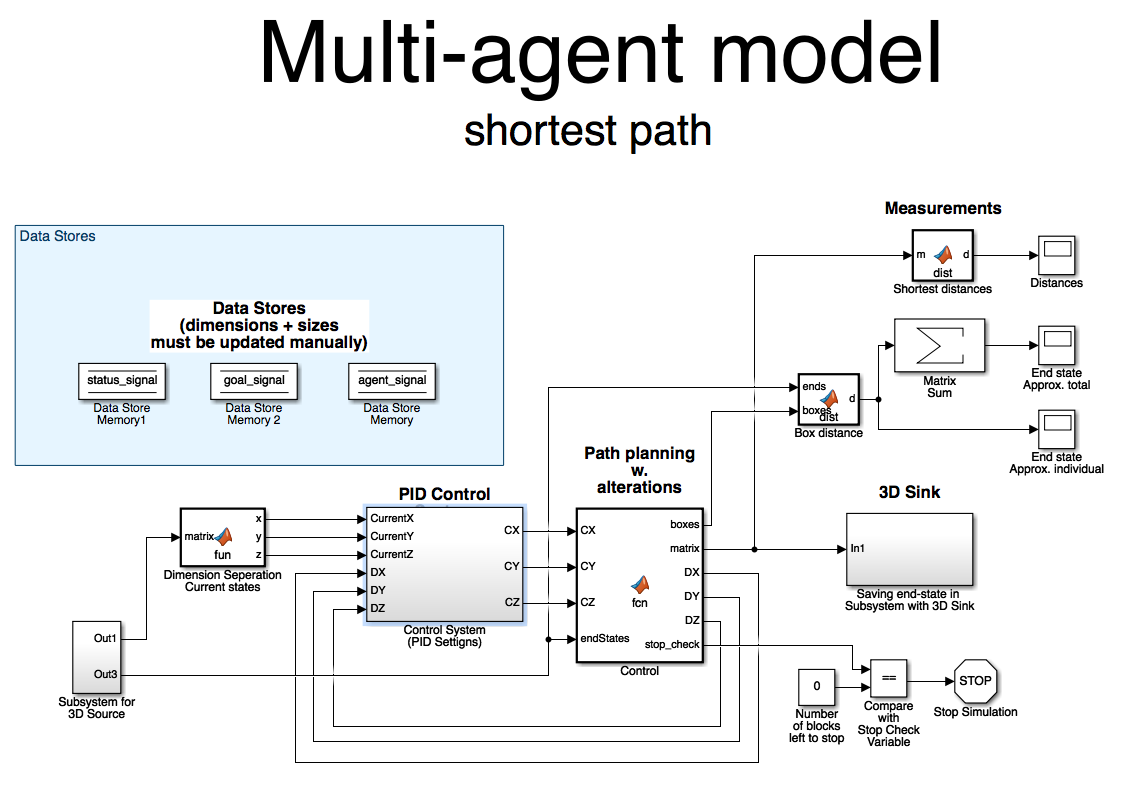
\includegraphics[width=1\columnwidth]{figures/model_overview}
  	\caption{\label{fig:model_overview}Overview of finished model in Simulink}
\end{figure}

The following subsections will outline how the different model requirements from Section \ref{sec:design}, were implemented in a step wise manner.

\subsection{VR3D, Sources and Sinks}
% TODO: reference
As shown in Figure \ref{fig:2d_overview}, the simulation environment has certain starting points for the boxes and agents, and a desired endpoint for the boxes. The 3D animation is created with the Simulink plugin VR3D [INSERT REFERENCE], which acts both as a source and a sink. The VR3D editor is used to map the starting points of the objects, as well as the shape, size and all other visual aspects of the 3D environment. The actual 3D visuals can be found in Figure \ref{fig:3d_overview} where the transparent boxes are not physical objects but simply show the desired structure of the grey boxes. The data from the 3D environment, is then sent as a signal to the simulink model and to the control algorithm, which alters the signal and sends it back into the VR3D block to create an animation. The subsystems of the model which hold the source and the sink can be seen in Figure \ref{fig:model_overview} whereas the contents of the sink, with the signal parsing, is shown in Figure \ref{fig:3d_sink}

% 3D World
\begin{figure}[H]
	\centering
	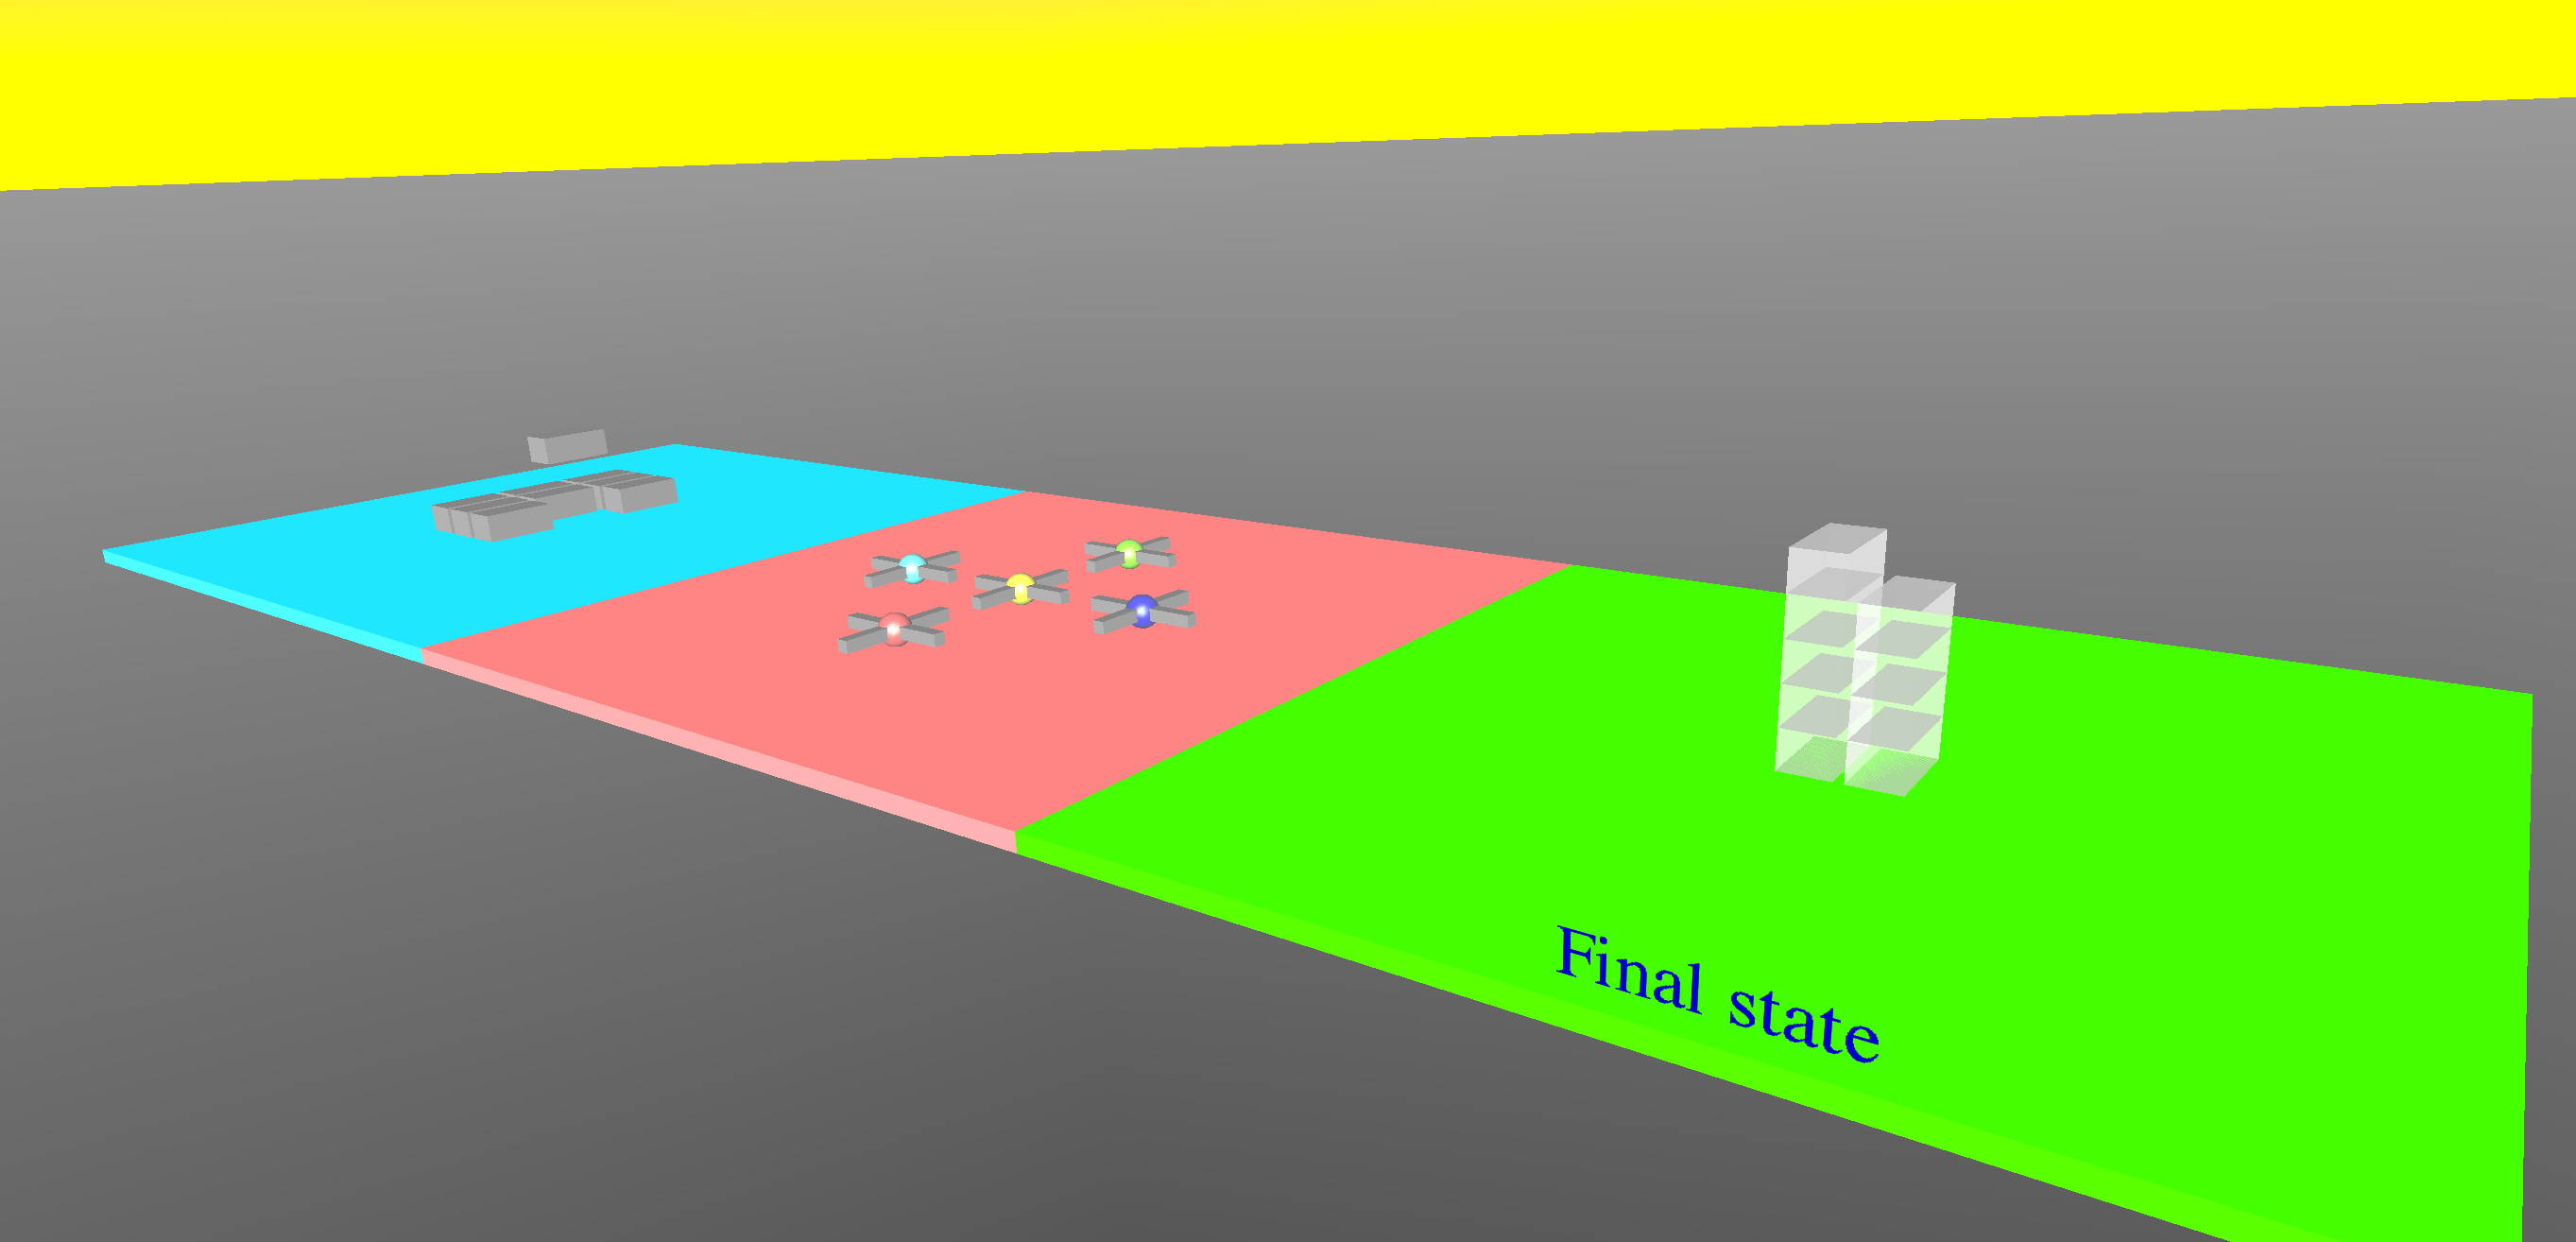
\includegraphics[width=1\columnwidth]{figures/3d_platform}
  	\caption{\label{fig:3d_overview}Screenshot from the VR3D environment used in the simulation}
\end{figure}

% 3D Sink
\begin{figure}[H]
	\centering
	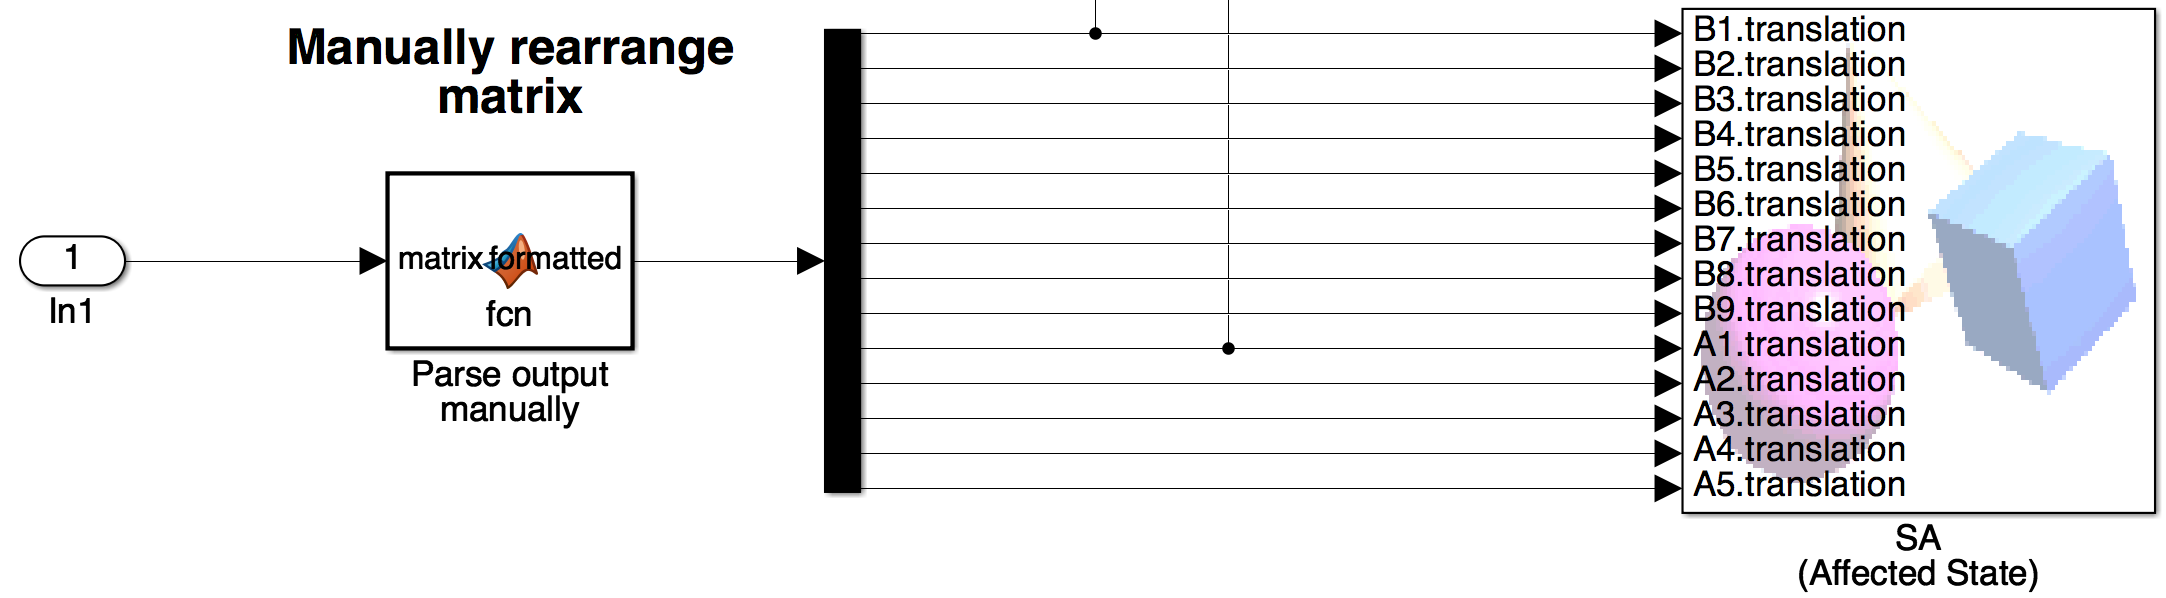
\includegraphics[width=1\columnwidth]{figures/3d_sink}
  	\caption{\label{fig:3d_sink}Signal from model being parsed to VR3D Sink}
\end{figure}



\subsection{PID Controller}
\label{sec:sim_pid}

As mentioned in Section \ref{sec:simulation_animation}, it is important the swarm control algorithm cannot alter the position of the agents directly, but instead give instructions to the quadcopters to change their thrust etc. Distribution of control is implemented by having two separate control systems as briefly mentioned in \ref{sec:agents}. The two systems are shown in Figure \ref{fig:3d_overview}, as blocks labeled \textbf{\texttt{Local Control}} and \textbf{\texttt{Global}}. 

The \textbf{\texttt{Global}} Control System, controls and navigates the agents using the desired swarm algorithm. This Control block os what is referenced to throughout this thesis, as the \textit{Control System}. 

%TODO: Reference
The \textbf{\texttt{Local Control}} is a subsystem (collection of Simulink blocks) responsible for handling the physical mechanics of the individual objects within the simulation. It uses a Simulink PID plugin, to enable the quadcopters to balance and move around in a real life manner. In practice, the global control system maps the different agents' desired position at a given time, sends this as a signal to the local control system. The local control system then attempts to achieve the results within the physical boundaries of the simulation [INSERT REFERENCE]. Figure \ref{fig:local_control} shows the local control system receiving the current and desired locations from the global control system, and for making the appropriate alterations.

% Local Control
\begin{figure}
	\centering
	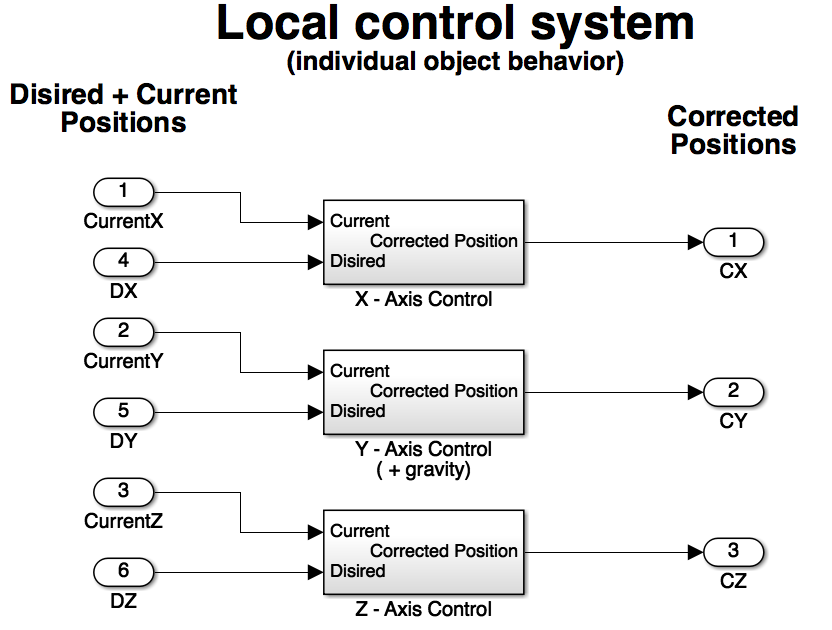
\includegraphics[width=.7\columnwidth]{figures/local_control}
  	\caption{\label{fig:local_control}Local Control subsystem}
\end{figure}

\subsection{Gravity \& Mass}
\label{sec:sim_gravity}

%TODO: Reference
The impulse of moving objects and their mass affected by gravity, is implemented within the Local Control System. This is done with a collection of Simulink blocks, which have been adjusted to enable real life object behavior based on newton mechanics [INSERT REFERENCE]. Figure \ref{fig:gravity_blocks} shows the model used to control behavior on the Y-Axis of the simulation (vertical), which includes the gravitational acceleration constant of ${9.8m/s^2}$. The models for the X+Z Axis are similar, with the difference of not having a constant acceleration.

% Gravity
\begin{figure}
	\centering
	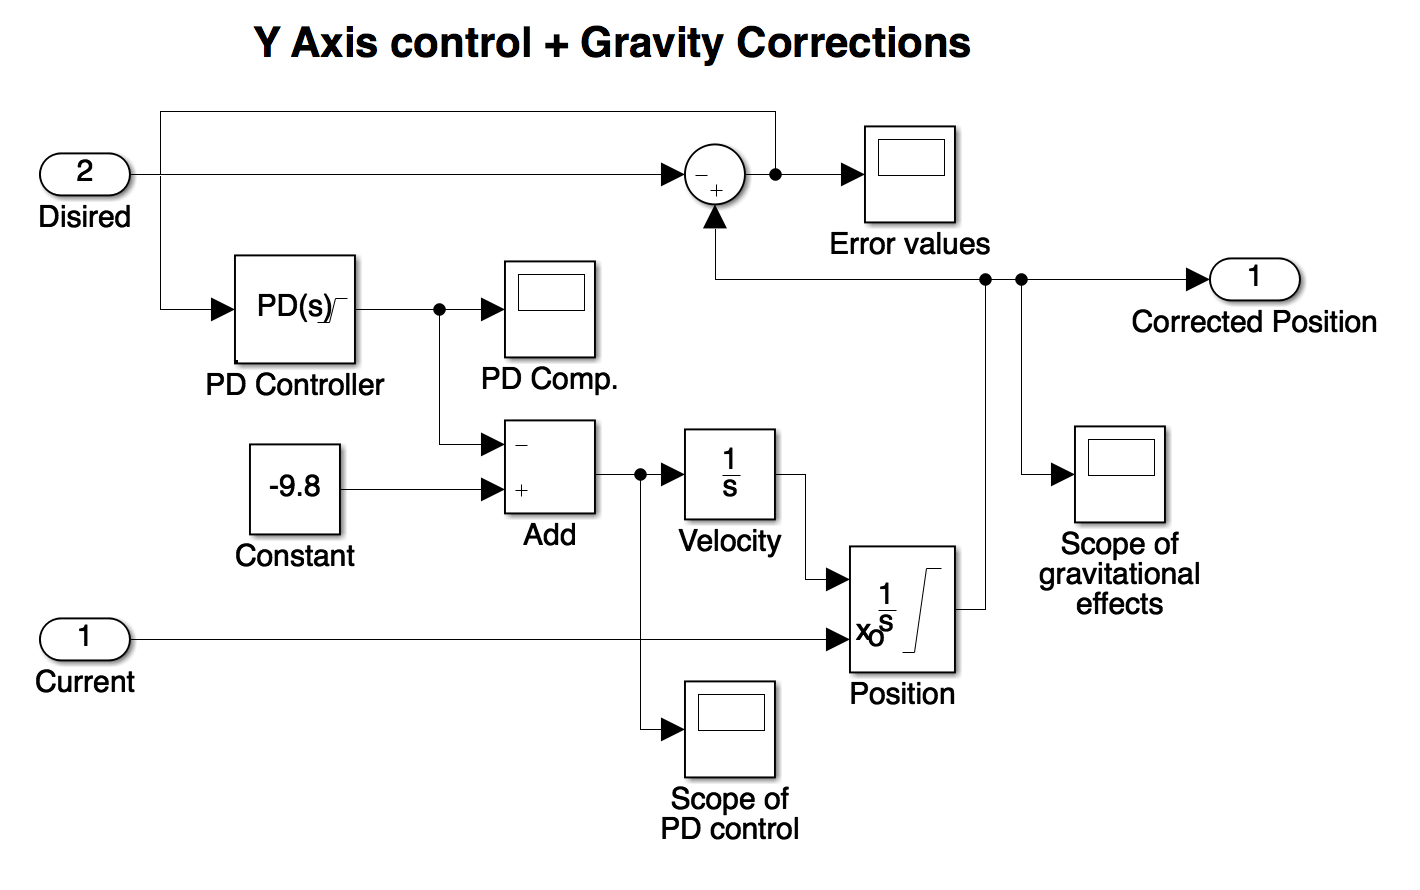
\includegraphics[width=.8\columnwidth]{figures/simulink_gravity_y}
  	\caption{\label{fig:gravity_blocks}Simulink model to implement physics mechanics on vertical axis}
\end{figure}

\subsection{Control Loop}

\subsection{Data Stores}

\subsection{Measurements}

\subsection{Completion Check}

\section{Validation}
\label{sec:validation}

Validation on single agent level

\subsection{Adjusting for desired behavior}
\label{sec:tuning}

% Pre adjustment
\begin{figure}[H]
  \centering
  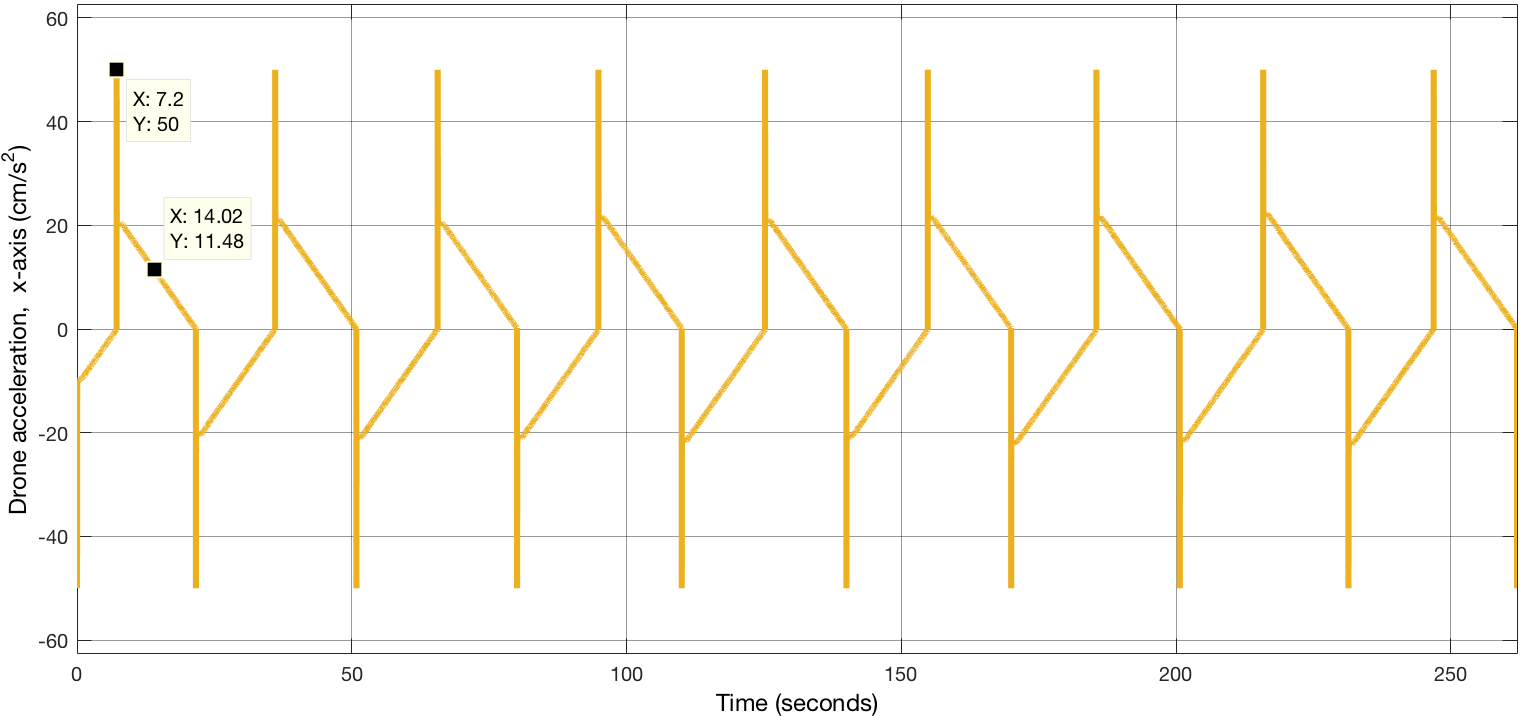
\includegraphics[width=1\columnwidth]{figures/SA_accel_pre_adjustment}
  \caption{\label{fig:pre_adjust}Agent acceleration before adjustment}
\end{figure}

Stable but too tall

% Post adjustment
\begin{figure}[H]
  \centering
  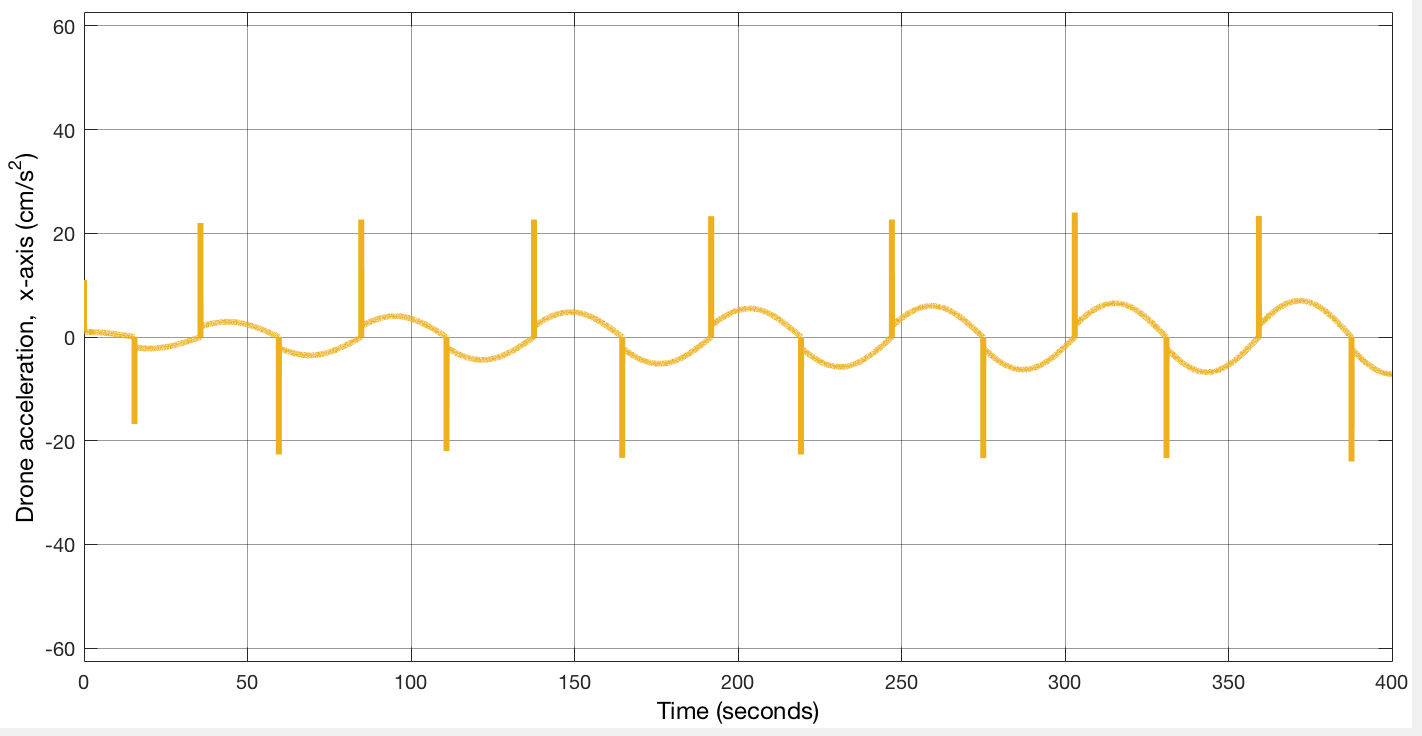
\includegraphics[width=1\columnwidth]{figures/SA_accel_pre_post_p_adjustment}
  \caption{\label{fig:post_adjust}Agent acceleration after adjustment of PD gains}
\end{figure}

short but unstable

% Post limitation
\begin{figure}[H]
  \centering
  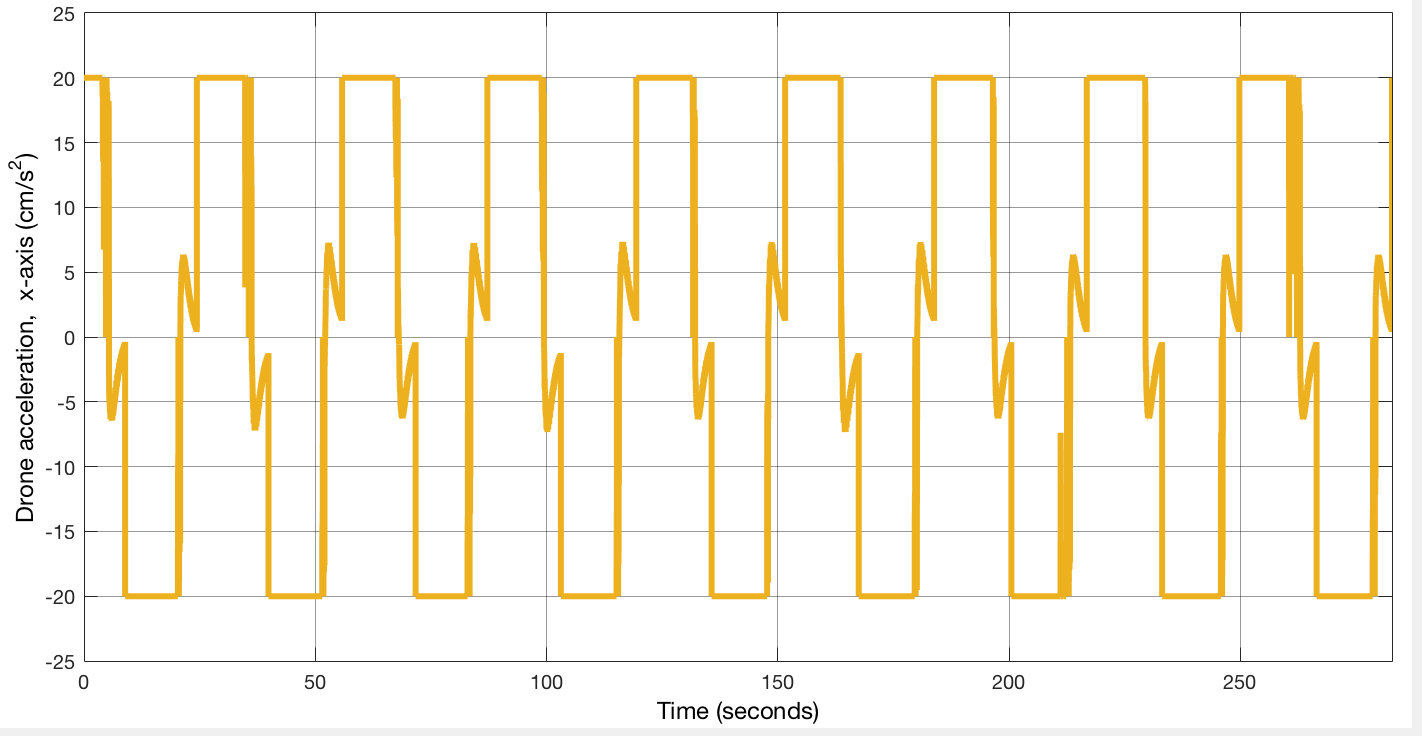
\includegraphics[width=1\columnwidth]{figures/SA_accel_post_final_adjustment}
  \caption{\label{fig:post_limit}Agent acceleration with acceleration}
\end{figure}

Shorter and wider is stable

\section{Test Metrics}
\label{sec:test_metrics}

\subsection{Testing on shortest path}



